    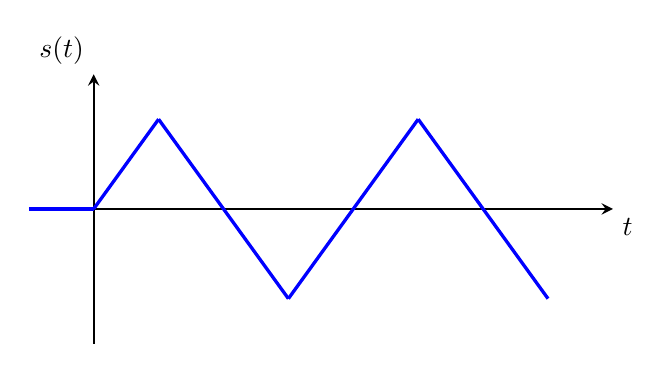
\begin{tikzpicture}
        \begin{axis}[
	ticks=none,
        axis line style = thick,
        height=5cm,
        width=9cm,
        axis x line=center,
        axis y line=center,
        xmin=-2,
        xmax=16,
        ymin=-1.5,
        ymax=1.5,
        xlabel={$t$},
        ylabel={$s(t)$},
        xlabel style={below right},
        ylabel style={above left},
        ]
        \addplot [very thick,color=blue,domain=-2:0, samples=101,unbounded coords=jump]{0};
        \addplot [very thick,color=blue,domain=0:2, samples=101,unbounded coords=jump]{0.5*x};
        \addplot [very thick,color=blue,domain=2:6, samples=101,unbounded coords=jump]{-0.5*x+2};
        \addplot [very thick,color=blue,domain=6:10, samples=101,unbounded coords=jump]{0.5*x-4};
        \addplot [very thick,color=blue,domain=10:14, samples=101,unbounded coords=jump]{-0.5*x+6};
        \end{axis}
    \end{tikzpicture}
